%%%%%%%%%%%%%%%%%%%%%%%%%%%%%%%%%%%%%%%%%%%%%%%%%%%%%%%%%%%%%%%%%
% Tese de Doutorado / Dept Fisica, CFM, UFSC                    %
% Andre@UFSC - 2014                                             %
%%%%%%%%%%%%%%%%%%%%%%%%%%%%%%%%%%%%%%%%%%%%%%%%%%%%%%%%%%%%%%%%%

%:::::::::::::::::::::::::::::::::::::::::::::::::::::::::::::::%
%                                                               %
%                          Capítulo 5                           %
%                                                               %
%:::::::::::::::::::::::::::::::::::::::::::::::::::::::::::::::%

%***************************************************************%
%                                                               %
%                        Decomposicao                           %
%                                                               %
%***************************************************************%

\chapter{Síntese de população estelar nas componentes morfológicas de galáxias}
\label{sec:Decomp}

%***************************************************************%
%                                                               %
%                      Seleção da amostra                       %
%                                                               %
%***************************************************************%

\section{Seleção da amostra}

\TODO: Amostra selecionada usando como critério: Candidata a S0 (descrever a
tabela de morfologia do CALIFA) e baixa inclinação (b/a > 0.6).

\TODO: Limpando a amostra. Ajustes iterativos de uma banda espectral, e inspeção
visual (primeira limpeza). Ajuste completo, e segunda inspeção visual.

\TODO: Criar tabela da amostra. Marcar quais foram vetadas em qual passo, e
escrever o motivo -- dust lane, bad fit, etc.

%***************************************************************%
%                                                               %
%                    Decomposicao bojo-disco                    %
%                                                               %
%***************************************************************%

\section{Decomposição morfológica}
\label{sec:Decomp:decomp}
 

\TODO Revisar esta seção. Neste trabalho trata-se apenas de galáxias com disco e
esferoidais.
Galáxias esferoidais seguem em geral um perfil de Sérsic, conforme a equação
\begin{equation*}
I(r) = I_e \exp \left\{- b_n \left[ \left( \frac{a}{r_e} \right)^{\sfrac{1}{n}}
- 1 \right] \right\}.
\end{equation*}
Já galáxias de tipo disco são bem modeladas por um perfil exponencial, dado por
\begin{equation*}
I(r) = I_0 \exp \left(- r / h \right).
\end{equation*}

Uma galáxia pode ser bem descrita como a soma de um disco exponencial e um bojo
com perfil de Sérsic. Através de um algoritmo de ajuste de funções, pode-se
determinar, dado o perfil de brilho de uma galáxia, qual combinação de valores
para os parâmetros livres (neste caso, $I_e$, $r_e$, $n$, $I_0$ e $h$) melhor
reproduz o perfil de brilho da galáxia.


%***************************************************************%
%                                                               %
%               Decomposição: decomposicao espectral            %
%                                                               %
%***************************************************************%

\section{Decomposição espectral}

O mesmo princípio foi então aplicado aos cubos de dados de IFS do CALIFA.
Diferente de do método de \citeauthor{Johnston2012}, foram ajustadas imagens a
cada comprimento de onda, utilizando um programa baseado na versão modificada do
Imfit, conforme a Seção \ref{sec:Decomp:decomp}. A decomposição é realizada
sobre os espectros sintéticos\fixme, provenientes de uma síntese realizada
anteriormente, sobre os dados originais. A motivação para isto é bastante
simples: evitar efeitos de linhas de emissão.
Estas seriam outra fonte de incerteza no ajuste morfológico, dado que em geral
estão relacionadas a regiões de formação estelar e núcleos ativos, que não
necessariamente seguem o mesmo perfil que o bojo ou o disco. Como este trabalho
é experimental, estas complicações foram deixadas de lado, neste momento.

\TODO: Explicar melhor o método de decomposição.

Os resultados apresentados aqui devem ser tomados com cuidado. O ajuste é feito
sem fazer hipótese alguma sobre como os parâmetros morfológicos variam a cada
comprimento de onda.


\subsection{Testes}

\TODO: Atualizar teste de decomposição. Mencionar os efeitos da PSF, discutidos
no próximo capítulo.

Para determinar se o método de decomposição funciona (ou melhor, se ele falha
mesmo para o caso mais básico), foi desenhado um exercício bastante simples.
Dado um conjunto de parâmetros morfológicos arbitrários, foi montado um cubo de
espectros de uma galáxia sintética composta de um bojo velho (utilizando uma SSP
de $12\,Gyr$) e um disco jovem (utilizando uma SSP de $3\,Gyr$). Os espectros de
base para o bojo e o disco podem ser vistos na Figura \ref{fig:testSpectra}.
Após gerar os cubos de dados de espectros, foi adicionado um ruído gaussiano de
$10\%$. Executando a decomposição neste cubo de dados simulado, deveria-se
encontrar valores para os parâmetros próximos aos escolhidos no início. A Figura
\ref{fig:testParameters} mostra a comparação dos parâmetros obtidos com os
iniciais. Os valores ajustados (linhas sólidas) estão de acordo com o valor
inicial, levando em conta o erro injetado nos espectros. É necessário repetir
este teste com configurações mais complexas, a fim de determinar as limitações
do método.


\begin{figure}
	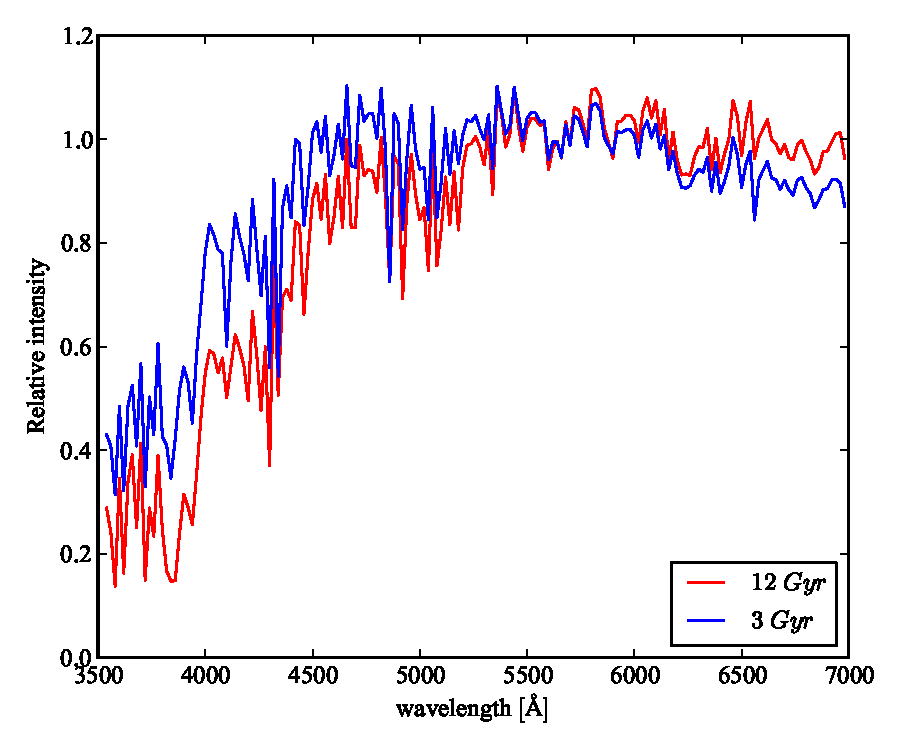
\includegraphics[width=0.7\columnwidth]{figuras/test-spectra}
	\caption[Espectros de base para o teste de decomposição] {Espectros de base
	para o teste de decomposição.}
	\label{fig:testSpectra}
\end{figure}


\begin{figure}
	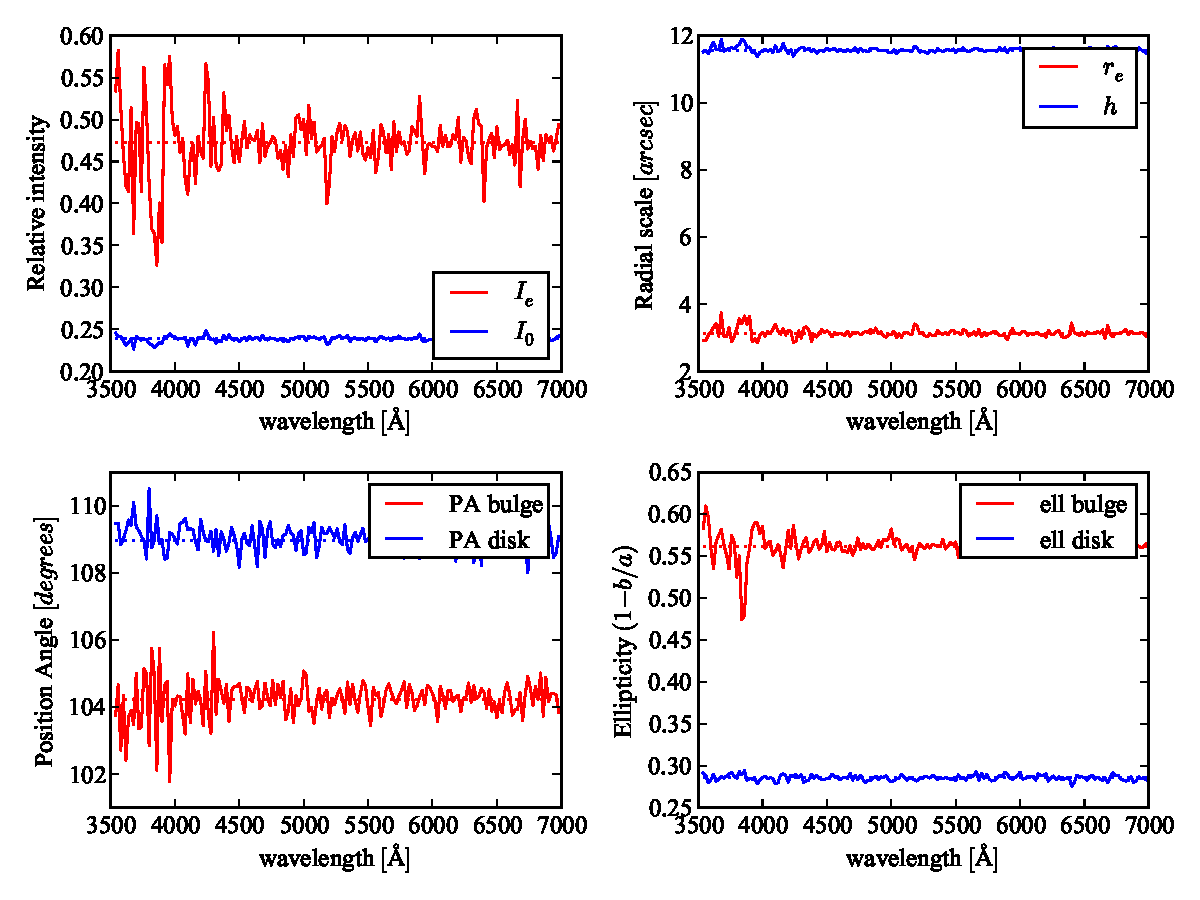
\includegraphics[width=1.0\columnwidth]{figuras/test-parameters}
	\caption[Parâmetros obtidos com o teste de decomposição] {Parâmetros obtidos
	com o teste de decomposição. Em tracejado são os parâmetros originais, em
	linhas sólidas os ajustes. Os parâmetros do bojo estão em vermelho e os do
	disco em azul. O índice de Sérsic ($n$) foi mantido constante e igual a $4$.}
	\label{fig:testParameters}
\end{figure}

\section{Resultado}

\TODO: Refazer todo o que vem a seguir.

A discussão a seguir refere-se à decomposição feita sobre os cubos de dados da
galáxia UGC 10695 (Figura \ref{fig:decompTarget}). A decomposição foi feita
utilizando a seguinte configuração:

\begin{figure}
	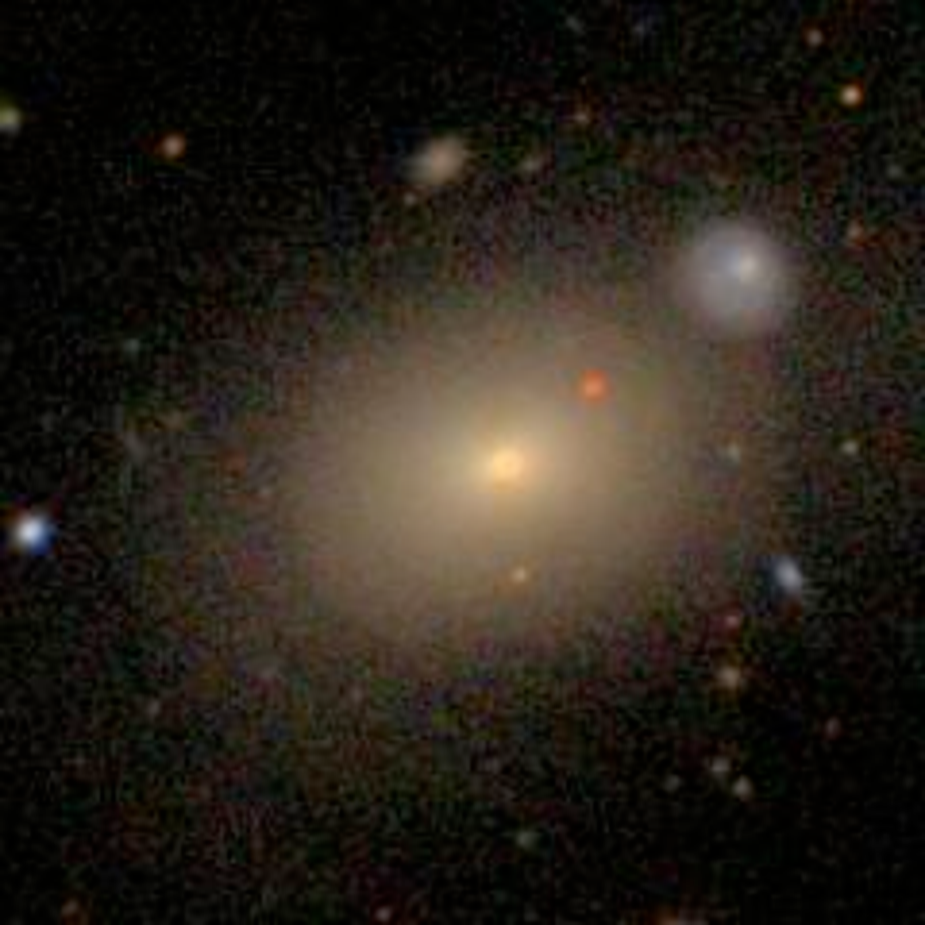
\includegraphics[width=0.3\columnwidth]{figuras/K0846}
	\caption[Montagem RGB da galáxia UGC 10695, do SDSS] {Montagem RGB da galáxia 
	UGC 10695, do SDSS.}
	\label{fig:decompTarget}
\end{figure}

\begin{itemize}

	\item Todos os pixels originais, sem agrupar em zonas de Voronoi.

	\item Espectros sintéticos provenientes de uma síntese executada anteriormente.

	\item Ajuste de todos os parâmetros livres: $I_e$, $r_e$, $n$, $I_0$, $h$ e a
	geometria da elipse\footnote{A geometria da elipse é definida pelo ângulo de
	posição ({\em P.A.}) e a elipticidade ($1 - b/a$).}.

	\item Convolução com uma PSF\footnote{{\em Point Spread Function}, a
	distribuição que representa a forma que uma fonte pontual aparece na imagem.}
	gaussiana de largura a meia altura de $2,4\,"$, medida numa estrela presente no
	campo observado.

\end{itemize}

Na Figura \ref{fig:decompParams} pode-se ver os parâmetros obtidos no ajuste
morfológico. Em comprimentos de onda menores que $4000\,\AA$ o ajuste sai um
pouco ruidoso, provavelmente devido à má calibração dos espectros do CALIFA
nesta região. Nas outras regiões os parâmetros tendem a variar suavemente,
embora haja variações locais próximas às linhas de absorção. Em especial, o
ângulo de posição do bojo e do disco, e o centro dos dois modelos, são
praticamente constantes.

A Figura \ref{fig:decompImages} permite uma visualização bidimensional dos
modelos em $5635\,\AA$, e uma comparação com a imagem original neste comprimento
de onda. O resíduo é mostrado no painel inferior direito. Ali se observa efeitos
de borda próximo às regiões externas mascaradas, além de um artefato no núcleo,
provavelmente devido à forma da PSF. Outra forma de visualizar a qualidade do
ajuste é através do perfil radial. A Figura \ref{fig:decompRadprof} mostra o
perfil radial em intervalos de aproximadamente $100\,\angstrom$. Ali se vê que o
disco e o bojo estão bem modelados, e que o ajuste é muito bom (o modelo é
marcado com uma linha preta pontilhada, e a sua maior parte fica sob a linha
preta sólida, o perfil original).

Os espectros obtidos são geralmente bem comportados. Um exemplo, a $5"$ do
núcleo, pode ser visto no painel superior da Figura \ref{fig:decompSpectra}.
O espectro de resíduo apresenta poucos artefatos. Nos painéis inferiores estão
os parâmetros de intensidade ($I_e$ e $I_0$) e de escala ($r_e$ e $h$), para
comparação.

\begin{figure}
	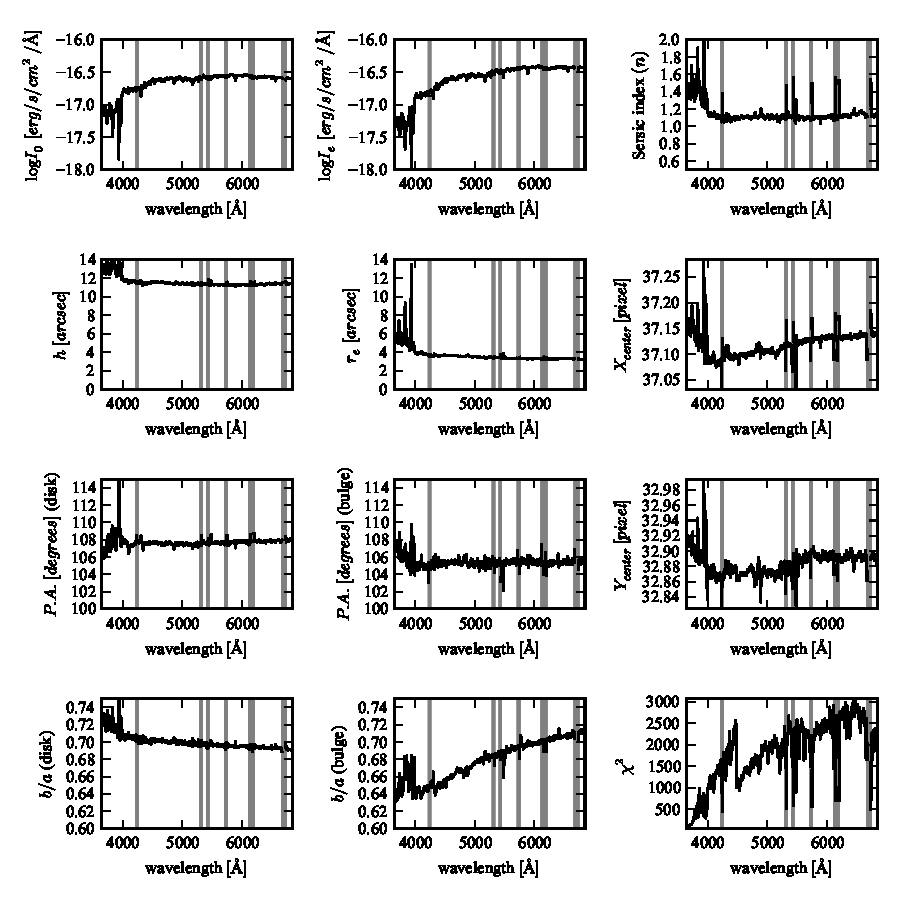
\includegraphics{figuras/decomp-fit-parameters}
	\caption[Parâmetros morfológicos] {Parâmetros morfológicos obtidos no ajuste
	de UGC 10695. Nos painéis à esquerda estão os parâmetros para o disco. Nos
	painéis ao centro, e no painel superior à direita, estãos os parâmetros do
	bojo. Ainda na coluna da direita há os painéis da posição do centro dos
	modelos e o $\chi^2$ do ajuste.}
	\label{fig:decompParams}
\end{figure}

\begin{figure}
	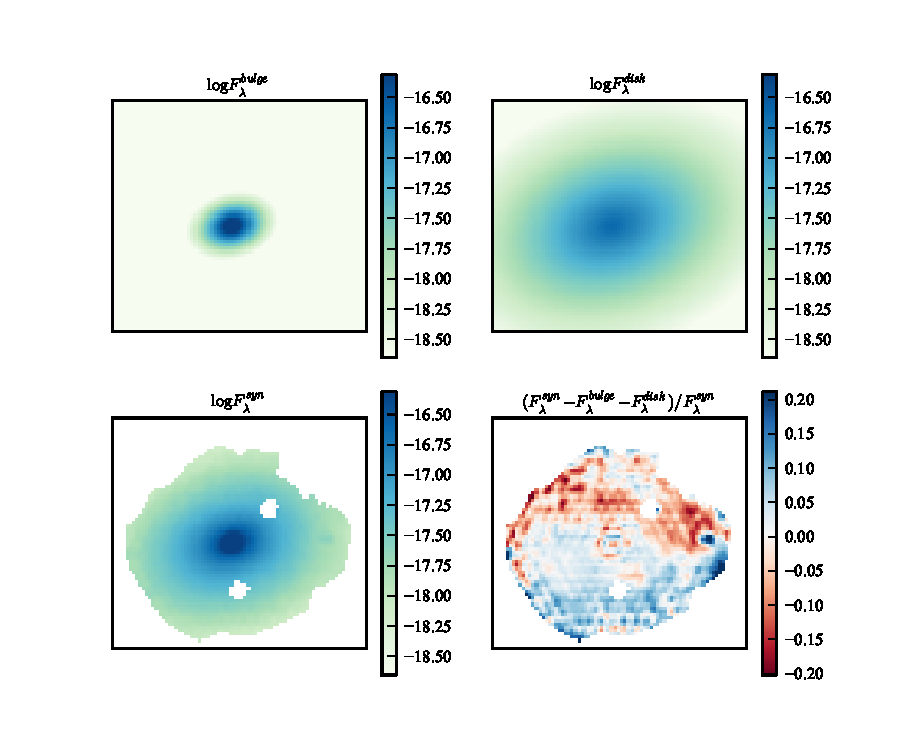
\includegraphics{figuras/decomp-model-images}
	\caption[Visualização 2-D da decomposição morfológica] {Visualização 2-D da
	decomposição morfológica. Nos painéis superiores os modelos de bojo e disco em
	$5635\,\angstrom$. No painel inferior à esquerda, a imagem original. No painel
	inferior à direita, o resíduo do ajuste, normalizado pela imagem original.}
	\label{fig:decompImages}
\end{figure}

\begin{figure}
	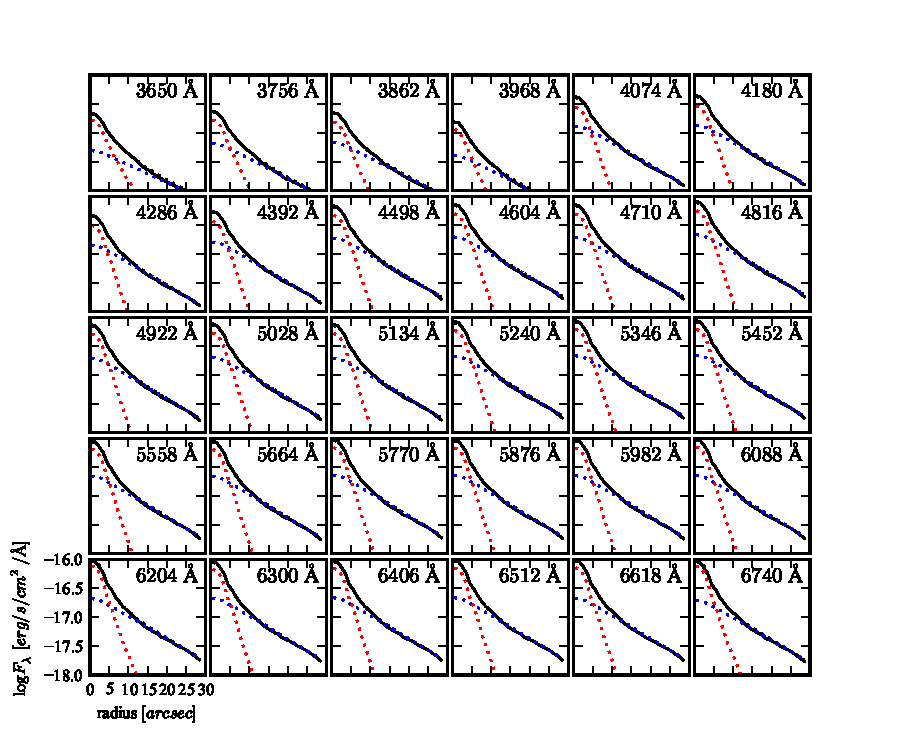
\includegraphics{figuras/decomp-radial-profile}
	\caption[Perfis radias da decomposição em função do comprimento de onda]
	{Perfis radias da decomposição em função do comprimento de onda.}
	\label{fig:decompRadprof}
\end{figure}

\begin{figure}
	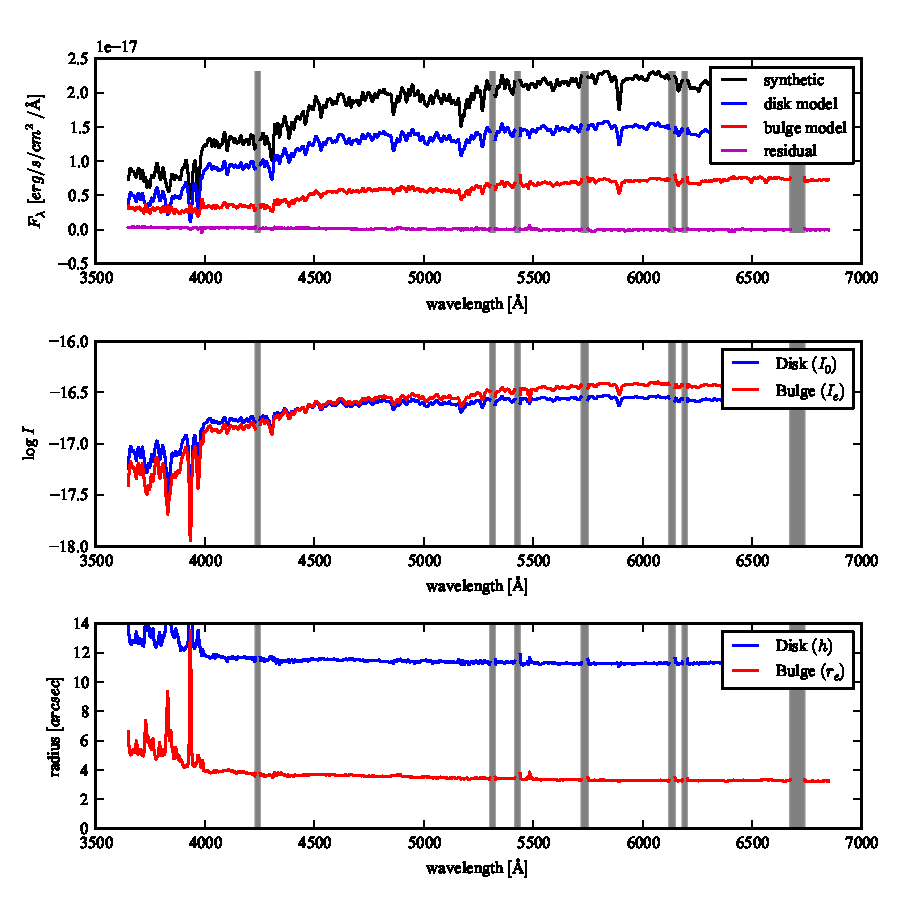
\includegraphics{figuras/decomp-model-quality}
	\caption[Espectro decomposto a $5"$ do núcleo] {Espectro decomposto a $5"$ do
	núcleo.}
	\label{fig:decompSpectra}
\end{figure}


%% End of this chapter
